\documentclass{standalone}
\usepackage{tikz}
\usepackage{hsbcommon}
\begin{document}
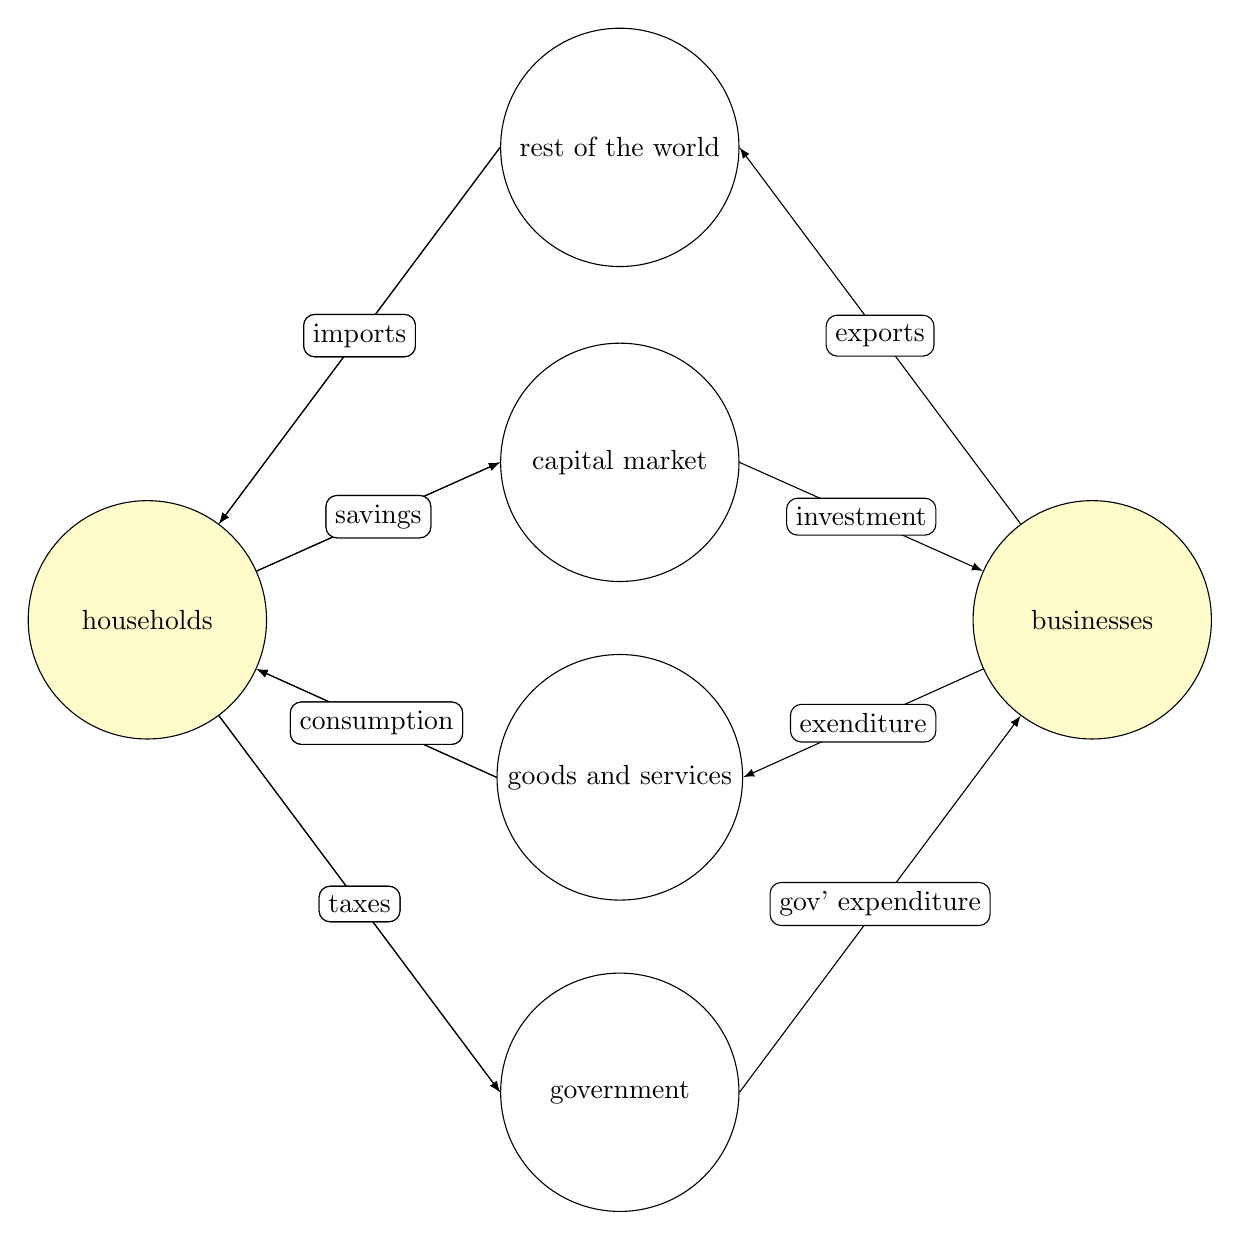
\begin{tikzpicture}
    \tikzset{%
        first/.style={%
            draw,
            fill=yellow!20,
            circle,
            rounded corners, 
            minimum width=20ex,
            minimum height=20ex
            },
        second/.style={
            draw, 
            circle,
            minimum width=20ex,
            },
        conn/.style={
            draw,
            rounded corners,
            fill=white
        },
        every path/.style={
            draw, >=latex
        }
    }
    \node[first] (HH) at (-6,0) {households};
    \node[first] (BN) at (6,0) {businesses};

    
    \foreach [count=\i] \connect/\in/\out/\dir in {
        government/taxes/gov' expenditure/->,
        goods and services/consumption/exenditure/<-,
        capital market/savings/investment/->,
        rest of the world/imports/exports/<-%
    }
    {
        \node[second] (C\i) at (0,4*\i-10) {\connect};
        \draw[\dir] (HH) to node[conn] {\in} (C\i.west);
        \draw[\dir] (HH) to node[conn] {\in} (C\i.west);
        \draw[\dir] (C\i.east) to node[conn] {\out} (BN);
        % node[conn] {\out} (BN);
    }
    % \draw (BN) to  node[conn] {income}    (HH);
    
\end{tikzpicture}
\end{document}
